\documentclass{standalone}
\usepackage{tikz}
\usetikzlibrary{matrix, positioning, calc}


\begin{document}




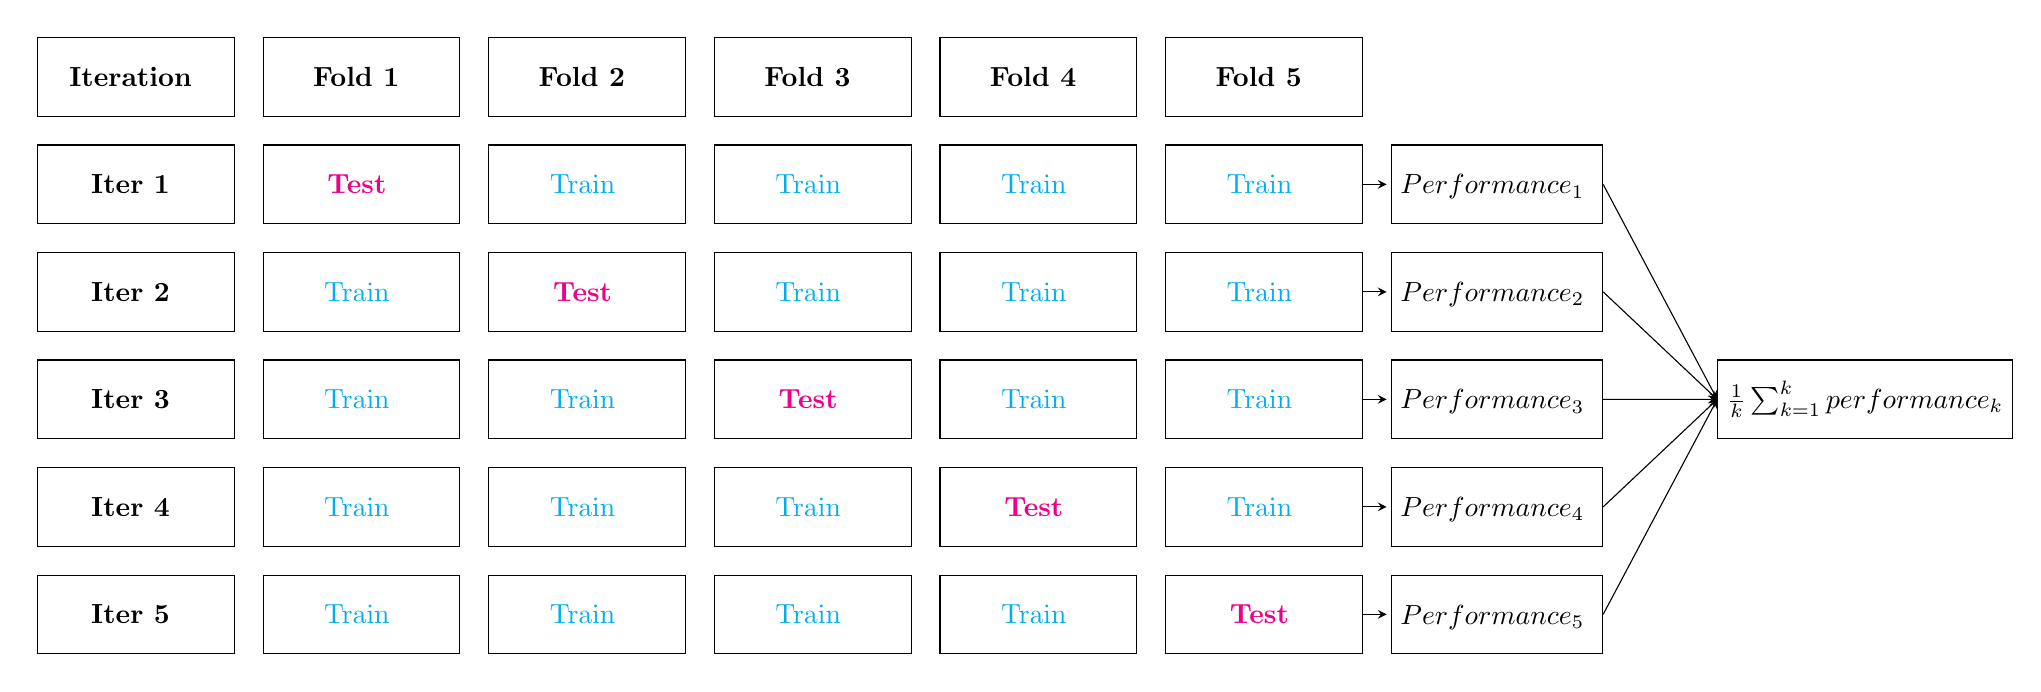
\begin{tikzpicture}[scale=10]

    % Create the matrix
    \matrix (m) [matrix of nodes, 
        nodes in empty cells,
        row sep=1em, column sep=1em,
        nodes={draw, minimum width=2.5cm, minimum height=1cm, anchor=center, align=center},
        row 1/.style={font=\bfseries},
        column 1/.style={font=\bfseries},
        row 1 column 2/.style={text=black},
        row 1 column 3/.style={text=black},
        row 1 column 4/.style={text=black},
        row 1 column 5/.style={text=black},
        row 1 column 6/.style={text=black},
        column 1/.style={font=\bfseries},
        nodes={text depth=0pt,anchor=center}
        ] 
    {
        Iteration & Fold 1 & Fold 2 & Fold 3 & Fold 4 & Fold 5 \\ 
        Iter 1 & \textbf{\textcolor{magenta}{Test}} & \textcolor{cyan}{Train} & \textcolor{cyan}{Train} & \textcolor{cyan}{Train} & \textcolor{cyan}{Train} & {$Performance_1$} \\
        Iter 2 & \textcolor{cyan}{Train} & \textbf{\textcolor{magenta}{Test}} & \textcolor{cyan}{Train} & \textcolor{cyan}{Train} & \textcolor{cyan}{Train} & {$Performance_2$} \\
        Iter 3 & \textcolor{cyan}{Train} & \textcolor{cyan}{Train} & \textbf{\textcolor{magenta}{Test}} & \textcolor{cyan}{Train} & \textcolor{cyan}{Train} & {$Performance_3$} \\
        Iter 4 & \textcolor{cyan}{Train} & \textcolor{cyan}{Train} & \textcolor{cyan}{Train} & \textbf{\textcolor{magenta}{Test}} & \textcolor{cyan}{Train} & {$Performance_4$} \\
        Iter 5 & \textcolor{cyan}{Train} & \textcolor{cyan}{Train} & \textcolor{cyan}{Train} & \textcolor{cyan}{Train} & \textbf{\textcolor{magenta}{Test}} & {$Performance_5$} \\
    };
    
    % Arrows
    \foreach \i in {2,3,4,5,6}
    \draw[-stealth] (m-\i-6.east) -- ++(0.03,0) node[right, align=center] {};

    \node[draw, minimum width=2.5cm, minimum height=1cm, anchor=west, align=center, right=4.5cm of m-4-6.east] (avg) {$\frac{1}{k}\sum_{k=1}^k performance_k$};

    \foreach \i in {2,3,4,5,6}
    \draw[-stealth] (m-\i-7.east) -- (avg.west);


\end{tikzpicture}

\end{document}